\documentclass[TP, noCustomPackages]{UPSTI_Document}
\usepackage{IUT_Annecy}
\usepackage{logos_iut}

% --- Git info (nécessite git et les hooks gitinfo2 activés) ---
\usepackage{gitinfo2} % génère gitHeadInfo.gin via hooks post-commit/checkout/merge
% Voir doc gitinfo2 pour activer les hooks une fois:
%   git config --local gitinfo2.enabled true
%   git info # ou copier les hooks fournis par le package
\newcommand{\sequence}{P}
\newcommand{\UPSTIsousTitreEnTete}{Hackathon 1}

\graphicspath{{images/}}



\discipline{Informatique}
\newcommand{\UPSTIidClasse}{1}
\newcommand{\UPSTItitreEnTete}{Informatique}


%\newcommand{\UPSTIsource}{Certaines images proviennent du site freepics.com}

\usepackage{listings}
\usepackage{xcolor}
\usepackage{amssymb} % pour \Box et \CheckedBox
\usepackage{makecell} % permet \makecell{...} avec des \\ dans une cellule
\renewcommand\arraystretch{1.2}

\lstdefinelanguage{bash}{
  alsoletter={-},           % autoriser "-" dans les mots-clés
  morekeywords={
    ls, cd, mv, cp, rm, mkdir, rmdir, echo, cat, less, head, tail,
    grep, find, chmod, chown, ps, kill, top, man, which, alias, export,
    ssh, scp, rsync, tar, gzip, gunzip, ping, curl, wget, zip, unzip, code
  },
  sensitive=true,           % sensible à la casse
  morecomment=[l]{\#},      % commentaires avec #
  morestring=[b]",          % chaînes "..."
  morestring=[b]'           % chaînes '...'
}

\definecolor{colString}{rgb}{0.6,0.1,0.1}
\definecolor{lightblack}{rgb}{0.3,.3,.3}

\newcommand{\prompt}[1]{\textcolor{gray}{#1}}

% \lstdefinestyle{console}{
%   language=bash,
%   basicstyle=\ttfamily,
%   columns=fullflexible,
%   keepspaces=true,
%   escapeinside=||, % <- permet d'injecter du LaTeX entre |...|
% }

\lstdefinestyle{console}{
    basicstyle      = \footnotesize\ttfamily,% ecriture standard
    extendedchars   = true,% permet d'avoir des accents dans le code
    tabsize         = 2,%
    showspaces      = false,%
    showstringspaces = false,%
    numbers=none,%
    breaklines=true,%
    breakautoindent=true,%
    escapeinside=|| % <- permet d'injecter du LaTeX entre |...|
}




\documentVersion{E}
\newcommand{\UPSTInumeroVersion}{\gitAuthorDate\if \gitDirty*dirty \fi}
\newcommand{\UPSTInumero}{\sequence}
\usepackage{eso-pic}
\begin{document}
% QR code (marqueur pédagogique) : superposition additive en bas à droite de chaque page via eso-pic.
% Le pied de page visible est dessiné par le package background (UPSTI_Templates) et les pieds fancyhdr
% ne s'affichent pas dans ce gabarit : on n'y touche donc pas.
%
% Image statique (sources/images/marqueur_qr.png), pas le package qrcode en
% direct : \qrcode{...} perd silencieusement les espaces et casse sur les
% caractères actifs du français (ex. ":") lors de sa réexpansion verbatim
% interne (testé : texte collé sans espaces, puis erreur fatale "Missing
% \endcsname inserted" selon la ponctuation). L'image a été générée avec
% qrencode (mode 8 bits, UTF-8) et son contenu vérifié par relecture
% automatique (décodage exact, caractère pour caractère) avant intégration
% -- fiable, contrairement à la génération TeX en direct.
%
% SOURCE UNIQUE DU TEXTE (à modifier ici seulement, jamais dans le .png ni
% en dupliquant ailleurs) : sources/images/marqueur_qr.txt -- lu tel quel
% par sources/aide.tex (texte blanc). Après modification de ce .txt,
% régénérer l'image depuis ce dossier (TD_01/) avec :
%   qrencode -8 -o sources/images/marqueur_qr.png -s 10 -l H \
%       -r sources/images/marqueur_qr.txt
% (paquet Debian/Ubuntu : qrencode. Si absent et sans accès root, le
% récupérer localement sans l'installer : `apt-get download qrencode
% libqrencode4` puis `dpkg-deb -x *.deb ./qrencode-local` et lancer le
% binaire extrait avec LD_LIBRARY_PATH pointant vers sa lib extraite.)
\AddToShipoutPictureFG{%
    \AtPageLowerLeft{\put(\LenToUnit{\paperwidth-1.1cm},\LenToUnit{0.35cm}){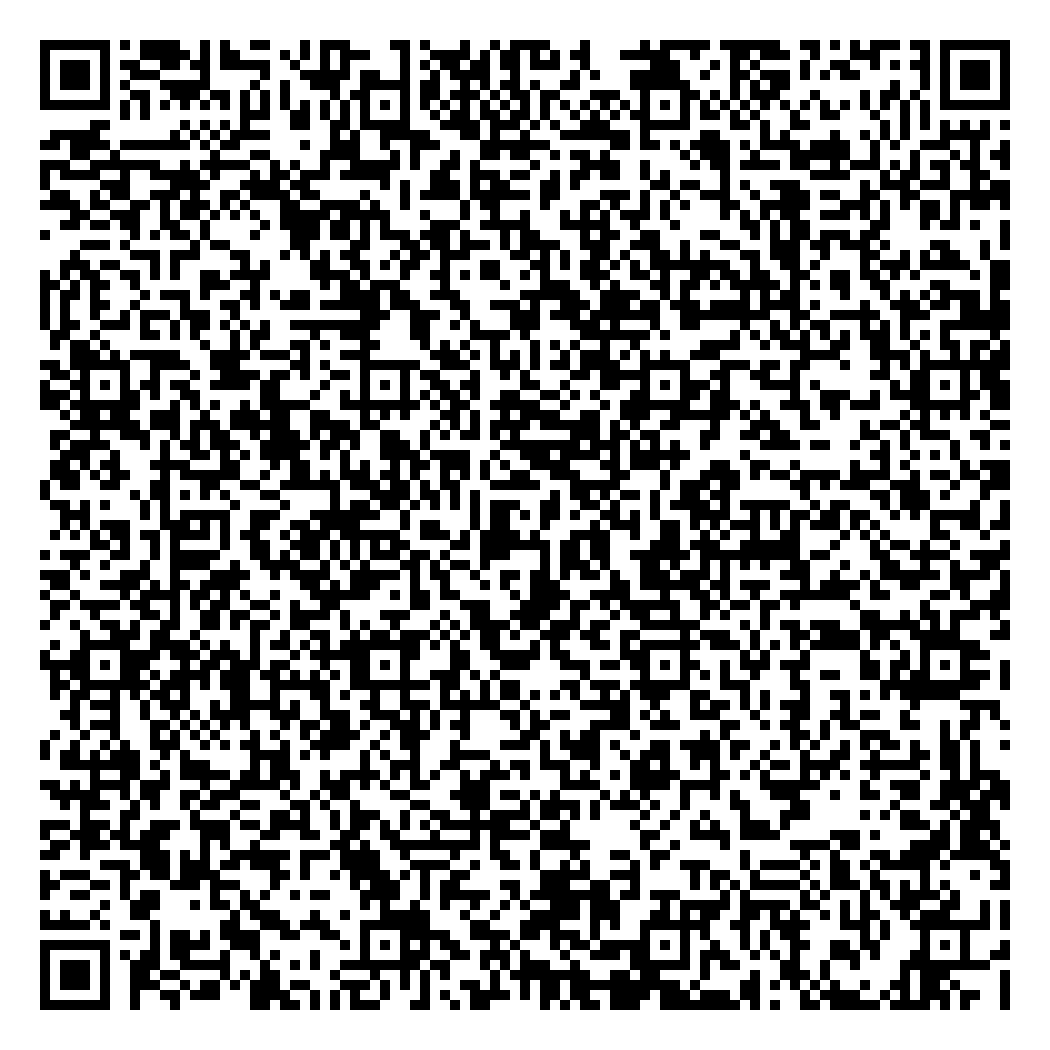
\includegraphics[height=0.7cm]{sources/images/marqueur_qr.png}}}%
}

% Même marqueur, en texte (pas juste en QR), répété en tout petit et en
% blanc sur CHAQUE page (pas seulement la section "aide" comme avant) --
% marge haute, hors de la zone d'en-tête UPSTI déjà imprimée. Toujours la
% même source unique sources/images/marqueur_qr.txt.
\AddToShipoutPictureFG{%
    \AtPageUpperLeft{\put(\LenToUnit{1.5cm},\LenToUnit{-1cm}){%
        \parbox{15cm}{\tiny\color{white}\input{sources/images/marqueur_qr.txt}}%
    }}%
}

\tableofcontents
\pagebreak
\section{Projet 1 — Le 421 simplifié}

\subsection*{Règles du jeu}
\begin{itemize}
  \item Le jeu se joue à deux joueurs.
  \item Chaque joueur dispose de 30 points au début de la partie.
  \item Le premier joueur lance trois dés.
  \item Il peut ensuite relancer un ou plusieurs dés, dans la limite de trois lancers au total.
  \item Il peut s’arrêter avant le troisième lancer s’il le souhaite.
  \item Le second joueur joue ensuite de la même manière et doit effectuer exactement le même nombre de lancers que le premier.
  \item À la fin de la manche, on compare les combinaisons. Le vainqueur prend à son adversaire un nombre de points dépendant de sa combinaison.
  \item Le vainqueur d’une manche commence la manche suivante.
  \item Le vainqueur final est celui qui a pris tous les points de son adversaire.
\end{itemize}

\subsection*{Contraintes imposées}
\begin{itemize}
  \item Les 3 dés du joueur 1 sont rangés dans les 3 \textbf{premières} cases d'un tableau \texttt{l\_tab\_jeu} de 6 cases ; ceux du joueur 2 dans les 3 \textbf{dernières} cases.
  \item Les points des 2 joueurs sont rangés dans un tableau de 2 cases.
  \item Un \textbf{seul} code gère aussi bien le joueur 1 que le joueur 2 (voir aide ci-dessous).
  \item Pour relancer des dés, le joueur indique leurs numéros sous la forme d'un entier (ex.\ \texttt{23} pour relancer les dés n°2 et n°3).
\end{itemize}

\subsection*{Combinaisons gagnantes}
Voici les combinaisons possibles, classées de la meilleure à la moins bonne :
\begin{center}
\begin{tabular}{|c|c|c|}
\hline
\textbf{Combinaison} & \textbf{Description} & \textbf{Points} \\ \hline
4--2--1 & Spéciale & \textbf{21} \\ \hline
Triplette & Trois dés identiques & Valeur du dé $\times 2$ \\ \hline
Paire & Deux dés identiques (le troisième départage) & Valeur du dé de la paire \\ \hline
Aucune & Le plus grand nombre formé l’emporte & 1 \\ \hline
\end{tabular}
\end{center}

\subsection*{Cahiers des charges}
\begin{UPSTICahierDesCharges}{Fonctionnement normal - Score manuel}
  Le programme
  \begin{itemize}
    \item Explique les règles
    \item Permet aux joueurs de jouer au jeu, en gérant les lancers et relances
    \item Seul le score de chaque manche n'est pas calculé automatiquement : 
    \begin{itemize}
      \item Le programme demande le vainqueur
      \item Le programme demande le nombre de points à transférer
    \end{itemize}
  \end{itemize}
\end{UPSTICahierDesCharges}

\begin{UPSTICahierDesCharges}{Score automatique}
  Le programme reconnaît la meilleure combinaison et gère les points lui-même.

  \textit{Aide :} pour reconnaître les combinaisons, il est conseillé de ranger les dés dans l'ordre croissant.
\end{UPSTICahierDesCharges}

\begin{UPSTICahierDesCharges}{L'ordinateur joue}
  Mode solo : jouer contre l'ordinateur.
\end{UPSTICahierDesCharges}

\begin{UPSTICahierDesCharges}{Idées d'améliorations} 
  \begin{itemize}
    \item Afficher les dés sous forme de carrés 
    \item Ajouter les combinaisons manquantes du vrai jeu 421
    \item Autres ?
  \end{itemize}
\end{UPSTICahierDesCharges}


\pagebreak
\section{Projet 2 — Le compte est bon}
\setcounter{UPSTInumeroCahier des charges}{0}

\subsection*{Objectif du jeu}
Obtenir une \textbf{cible} comprise entre 100 et 999 en combinant \textbf{six nombres tirés} dans une liste donnée, à l’aide des opérations $+,-,\times,/$ (division exacte uniquement).

\subsection*{Règles du jeu}
\begin{itemize}
  \item Six nombres sont tirés au hasard dans la liste officielle : deux occurrences de 1 à 10, puis 25, 50, 75, 100.
  \item Une \textbf{cible} aléatoire entre 100 et 999 est annoncée.
  \item Chaque nombre peut être utilisé \textbf{au plus une fois}.
  \item Les opérations autorisées sont $+,-,\times,/$ et les divisions doivent être \textbf{entières}.
  \item Une manche dure \textbf{60 secondes} (vous pouvez réduire à 3 s pour les tests).
\end{itemize}

\subsection*{Cahiers des charges} 
\begin{UPSTICahierDesCharges}{Jeu simple}
\begin{itemize}
  \item  Tirage des \textbf{6 nombres} et d'une \textbf{cible} puis affichage.
  \item A la fin du temps, le joueur \textbf{annonce} s'il a réussi ou non.
  \item S'il a réussi, il gagne un point. Sinon, il perd un point (il ne peut pas avoir de points négatifs).
  \item Le joueur gagne s'il atteint 3 points.
\end{itemize}

\textit{Aide :} utilisez \texttt{srand(time(NULL))}, \texttt{rand()} et \texttt{\%} pour borner les tirages ; un chronométrage simple peut se faire avec \texttt{time(NULL)} et une boucle d'attente.
\end{UPSTICahierDesCharges}

\begin{UPSTICahierDesCharges}{Tirage sans remise}
  \begin{itemize}
    \item Tirage \textbf{sans remise} à partir du tableau de 24 valeurs (respect des probabilités).
  \end{itemize}
On considère que les nombres sont tirés à partir d'un panier dans lequel les balles ne sont pas replacées après tirage. Ainsi, si, par exemple, un 5 est tiré, il n'en reste plus qu'un au lieu de deux dans le panier. 

En programmation, cela revient à tirer au sort dans le tableau et à ne plus pouvoir tirer la case au sort. 

\textit{Proposition de technique :} \og \textbf{swap avec la dernière case}\fg{} : lorsqu'une case est choisie, copiez la dernière case à sa place et réduisez la borne de tirage (24 $\rightarrow$ 23 $\rightarrow$ …). Par exemple, si au premier tirage (sur 24 cases) la case n°15 est choisie, on l'écrase avec le contenu de la dernière case ; le tirage suivant se fait sur 23 cases \textit{(voir section~\ref{sec:tirage-sans-remise})}.

Il est conseillé de travailler sur un \textbf{tableau image}, réinitialisé avec le tableau de base à chaque nouvelle partie.
\end{UPSTICahierDesCharges}

\begin{UPSTICahierDesCharges}{Saisie des opérations}
\begin{itemize}
  \item L'ordinateur affiche les nombre disponibles et le résultat à obtenir
  \item Le joueur saisit les opérations au clavier : deux entiers, puis le caractère de l'opération (\texttt{'+'}, \texttt{'-'}, \texttt{'*'}, \ldots) ; il saisit \texttt{-1} s'il n'a pas su faire le compte
  \item Après chaque opération, l'ordinateur retire les nombres déjà utilisés et affiche les nouveau nombres disponibles (résultats de l'opération). Par exemple : 
  \begin{enumerate}
    \item Cible : 645, avec 50, 6, 7, 1, 5, 2
    \item Le joueur saisit l'opération 6 + 7
    \item Cible : 645, avec 50, 13, 0, 1, 5, 2
    \item Le joueur saisit l'opération 50 * 13
    \item Cible : 645, avec 650, 0, 0, 1, 5, 2
    \item Le joueur saisit l'opération 650 - 5 : l'ordinateur affiche \og Le compte est bon !!! \fg{}
  \end{enumerate}
  \item Si la cible est atteinte, l'ordinateur affiche \textbf{Le compte est bon}
\end{itemize}  
\end{UPSTICahierDesCharges}
\begin{UPSTICahierDesCharges}{Améliorations possibles}
\begin{itemize}
  \item Affichage du compte à rebours
  \item ...
\end{itemize}  

\end{UPSTICahierDesCharges}


\pagebreak 
\section{Projet 3 — Bataille navale}
\setcounter{UPSTInumeroCahier des charges}{0}

\subsection*{Objectif du jeu}
Couler les bateaux cachés dans une \textbf{mer 6$\times$6} en proposant des \textbf{coordonnées} de tir. Le jeu se joue \textbf{joueur vs processeur}.

\subsection*{Règles du jeu}
\begin{itemize}
  \item La mer est une grille 6$\times$6.
  \item Deux bateaux : \textbf{Bateau n°1} (2 cases) et \textbf{Bateau n°2} (3 cases).
  \item Les bateaux sont placés \textbf{aléatoirement}, \textbf{horizontalement ou verticalement}, sans chevauchement et entièrement dans la grille.
  \item Le joueur propose des coordonnées. \textbf{Touché} si la case contient un bateau, \textbf{Coulé} lorsque toutes les cases d’un même bateau sont touchées.
  \item \textbf{Victoire} quand les deux bateaux sont coulés ; afficher le \textbf{nombre de tentatives} et le \textbf{temps de jeu}.
\end{itemize}

\subsection*{Codage conseillé des cases (pour la logique interne)}
\begin{center}
\begin{tabular}{|c|c|}
\hline
\textbf{Valeur} & \textbf{Signification} \\ \hline
0 & Case vide \\ \hline
1 & Bateau n°1, non touchée \\ \hline
10 & Bateau n°1, touchée \\ \hline
2 & Bateau n°2, non touchée \\ \hline
20 & Bateau n°2, touchée \\ \hline
\end{tabular}
\end{center}

\subsection*{Cahiers des charges}
\begin{UPSTICahierDesCharges}{Grille, placement et tirs}
\begin{itemize}
  \item Le joueur joue contre l'ordinateur et tente de couler ses bateaux.
  \item La mer doit être affichée après chaque tir, avec les cases déjà tirées marquées (Tirées vides / Touchées).
\end{itemize}
\end{UPSTICahierDesCharges}

\begin{UPSTICahierDesCharges}{Deux joueurs}
Un joueur place les bateaux, l'autre tente de les couler. Alterner les rôles.
\end{UPSTICahierDesCharges}

\begin{UPSTICahierDesCharges}{Deux joueurs}
Le vrai jeu. Chaque joueur place ses bateaux en début de partie (sans les montrer à l'autre). Les joueurs jouent à tour de rôle, chacun tentant de couler les bateaux adverses. 
\end{UPSTICahierDesCharges}


\pagebreak
\section{Projet 4 — Jeu Simon}
\setcounter{UPSTInumeroCahier des charges}{0}

\subsection*{Objectif du jeu}
Tester la mémoire des joueurs en construisant une \textbf{séquence de caractères} de plus en plus longue. À chaque tour, le joueur courant doit reproduire la séquence précédente puis \textbf{ajouter un nouveau caractère}.

\subsection*{Règles du jeu}
\begin{itemize}
  \item Le jeu se joue à deux personnes qui jouent en alternance, ou contre l’ordinateur.
  \item Le premier joueur saisit un \textbf{caractère minuscule} affiché à l’écran.
  \item Le second joueur doit alors saisir la même séquence \textbf{plus} un nouveau caractère. \textbf{Seul le dernier caractère saisi est affiché}. Si la séquence est incorrecte, il perd et le jeu s’arrête.
  \item Si la séquence du second joueur est juste, on repasse la main au premier joueur, et ainsi de suite : à chaque tour, on \textbf{rejoue la séquence complète} puis on ajoute un caractère.
  \item Deux offres de jeu : \textbf{Jeu 1} (2 joueurs physiques) ; \textbf{Jeu 2} (contre l’ordinateur, on affiche le \textbf{nombre de coups} en fin de partie).
\end{itemize}

\subsection*{Cahier des charges}
\begin{UPSTICahierDesCharges}{Séquence à deux joueurs}
\begin{itemize}
  \item Gérer la construction de la séquence \textbf{commune} (longueur max 50) et l’alternance des joueurs.
  \item À chaque tour : reproduire la séquence précédente, puis saisir \textbf{un nouveau caractère} (afficher uniquement le \textbf{dernier} caractère saisi).
  \item En cas d’erreur de séquence, \textbf{annoncer le perdant} et arrêter la partie.
\end{itemize}
\textit{Aide :} une \textbf{seule boucle} pour les deux joueurs (même code) avec une variable de joueur (\texttt{0/1}) ; afficher la séquence courante en parcourant le tableau de 0 à \texttt{nbrCoup}.
\end{UPSTICahierDesCharges}


\begin{UPSTICahierDesCharges}{Robustesse et présentation}
  \begin{itemize}
    \item Valider les saisies (lettre minuscule), gérer la \textbf{taille max} de 50 caractères et les \textbf{messages} de statut.
    \item Proposer un \textbf{menu} : Jeu 1 (2 joueurs) / Jeu 2 (contre l’ordinateur).
    \item Soigner l'affichage (Rendre le jeu le plus beau possible) 
  \end{itemize}
\end{UPSTICahierDesCharges}

\begin{UPSTICahierDesCharges}{Mode contre l’ordinateur}
\begin{itemize}
  \item L’ordinateur joue en alternance avec le joueur humain et \textbf{ajoute} un caractère à la séquence.
  \item En fin de partie, afficher le \textbf{nombre de coups} joués.
  \item Prévoir \textbf{plusieurs niveaux de difficulté} (fréquence d’erreurs de l’IA).
\end{itemize}
\textit{Aide :} générer le caractère de l’ordinateur aléatoirement, et introduire une \og erreur \fg{} selon une probabilité paramétrable.
\end{UPSTICahierDesCharges}


\pagebreak
\section{Projet 5 — Jeu des couleurs}
\setcounter{UPSTInumeroCahier des charges}{0}

\subsection*{Objectif du jeu}
L’ordinateur tire une \textbf{suite de 10 couleurs} parmi \textit{noir, vert, rouge, bleu}. Les couleurs s’affichent brièvement, puis disparaissent. Le joueur doit \textbf{reproduire la séquence} dans le bon ordre (codage numérique). Le score et la durée sont affichés en fin de partie. Un mode 2 joueurs est ensuite proposé.

\subsection*{Règles du jeu}
\begin{itemize}
  \item L'ordinateur choisit 10 couleurs au hasard parmi \{noir, vert, rouge, bleu\}. 
  \item Les 10 carrés de couleurs s'affichent en ligne pendant 5\,s, puis l’écran est effacé.
  \item Le joueur saisit la séquence en codes : \texttt{0} pour noir, \texttt{1} pour bleu, \texttt{2} pour vert, \texttt{3} pour rouge.
  \item À chaque saisie correcte, \textbf{+1 point}. À chaque erreur, \textbf{-1 point}.
  \item En fin de partie : Afficher le \textbf{score}.
\end{itemize}

\subsection*{Cahier des charges}
\begin{UPSTICahierDesCharges}{Mode 1 joueur simplifié}
\begin{itemize}
  \item Affichage de la séquence, puis effacement de l'écran
  \item Le joueur tente de reformer la suite
  \item Affichage du score en fin de partie.
\end{itemize}
\textit{Aide :} utiliser \texttt{srand(time(NULL))}, \texttt{rand()\%4}, \texttt{sleep(5)}, \texttt{system("clear")}; ANSI \texttt{\textbackslash033[40m..\textbackslash033[0m} pour les carrés.
\end{UPSTICahierDesCharges}

\begin{UPSTICahierDesCharges}{Mode 1 joueur complet}
\begin{itemize}
  \item A la fin de la partie, la séquence originale et la séquence du joueur sont affichées pour comparaison
  \item La durée et le score sont également affichés
\end{itemize}
\end{UPSTICahierDesCharges}

\begin{UPSTICahierDesCharges}{Mode 2 joueurs et bilan complet}
\begin{itemize}
  \item Chaque joueur saisit sa propre \textbf{séquence} ; comparer les scores et \textbf{annoncer le vainqueur}.
  \item Afficher les \textbf{trois séquences} : tirage, joueur~1, joueur~2, ainsi que leurs scores et durées.
  \item Soigner la \textbf{présentation} (espaces, retours à la ligne, lisibilité des carrés).
\end{itemize}
\textit{Aide :} réutiliser l’affichage des carrés et une fonction de calcul de score pour éviter la duplication.
\end{UPSTICahierDesCharges}


\pagebreak
\section{Projet 6 — Poker}
\setcounter{UPSTInumeroCahier des charges}{0}

\subsection*{Objectif du jeu}
Construire un jeu simplifié de Poker à 5 cartes pour un joueur, reconnaître les combinaisons demandées et calculer un score. Étendre ensuite à deux joueurs.

\subsection*{Règles du jeu}
\begin{itemize}
  \item On joue avec un \textbf{jeu de 32 cartes} (valeurs 7,8,9,10, V, D, R, As) et 4 couleurs.
  \item Le joueur reçoit \textbf{5 cartes} tirées au hasard \textbf{sans remise}. Il peut remplacer une ou plusieurs cartes.
  \item Combinaisons gagnantes : \textbf{paire} (+1), \textbf{brelan} (+2), \textbf{full} (+3), \textbf{carré} (+5).
  \item Afficher la main et la combinaison gagnante éventuelle. En version deux joueurs, \textbf{la meilleure main gagne}.
\end{itemize}

\subsection*{Codage des cartes}
Le jeu est un tableau \texttt{l\_tab\_jeu32} de 32 entiers (voir aide) : centaines = couleur (72 = \texttt{'H'} c\oe{}ur, 80 = \texttt{'P'} pique, 84 = \texttt{'T'} trèfle, 67 = \texttt{'C'} carreau), unités = valeur (7, 8, 9, 10, 11 valet, 12 dame, 13 roi, 1 as). La main du joueur est rangée dans un second tableau \texttt{l\_tab\_jeu5} de 5 entiers.

\subsection*{Cahier des charges}
\begin{UPSTICahierDesCharges}{Jeu de base}
\begin{itemize}
  \item Tirer \textbf{5 cartes sans remise} depuis le jeu de 32 cartes, les afficher (couleur et valeur).
  \item Permettre au joueur d’indiquer les cartes à remplacer (ex.\,un entier \texttt{134} pour 1,3,4), puis \textbf{re\-tirer} sans remise.
  \item Afficher la main finale.
\end{itemize}
\textit{Aide :} tirage sans remise : si au premier tirage (sur 32 cases) la case n°19 est choisie, on remplace son contenu par celui de la dernière case ; le tirage suivant se fait sur 31 cases, et ainsi de suite \textit{(voir section~\ref{sec:tirage-sans-remise})}.

\textit{Conseil :} pour tester, remplacez le tirage aléatoire par un tirage non aléatoire donnant une main gagnante.
\end{UPSTICahierDesCharges}

\begin{UPSTICahierDesCharges}{Score automatique}
\begin{itemize}
  \item Détecter automatiquement : \textbf{paire}, \textbf{brelan}, \textbf{full}, \textbf{carré} et \textbf{calculer le score}.
  \item Afficher un \textbf{récapitulatif} clair (main, combinaison, score).
  \item Vérifier la \textbf{saisie} des cartes à remplacer.
\end{itemize}
\textit{Aide :} ranger les valeurs des 5 cartes, compter les occurrences.
\end{UPSTICahierDesCharges}

\begin{UPSTICahierDesCharges}{Mode deux joueurs}
\begin{itemize}
  \item Mode \textbf{deux joueurs} : chacun joue sa main, comparaison des combinaisons et \textbf{annonce du vainqueur}.
  \item Présentation soignée, possibilité de \textbf{rejouer} plusieurs manches.
\end{itemize}
\end{UPSTICahierDesCharges}


\pagebreak
\section{Projet 7 — Le morpion}
\setcounter{UPSTInumeroCahier des charges}{0}

\subsection*{Objectif du jeu}
Réaliser un morpion (3×3) jouable à deux joueurs au clavier, avec affichage ASCII et détection de victoire/égalité.

\subsection*{Règles du jeu}
\begin{itemize}
  \item Affichage de la grille dans le terminal avec des caractères de base : \texttt{'X'} pour le joueur 1, \texttt{'O'} pour le joueur 2.
  \item Les joueurs jouent à tour de rôle tant que 3 caractères ne sont pas alignés. C'est le programme qui vérifie les alignements.
  \item Si un joueur joue sur une case inexistante ou déjà occupée, il \textbf{perd son tour}.
  \item Le jeu se joue avec le \textbf{pavé numérique} du clavier.
  \item En mémoire, la grille est un tableau de \textbf{9 entiers} : \texttt{0} = case vide, \texttt{1} = 'X' (J1), \texttt{2} = 'O' (J2).
\end{itemize}

\begin{center}
  \begin{minipage}{0.45\textwidth}
    \centering
    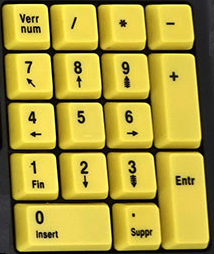
\includegraphics[width=0.8\textwidth]{sources/images/clavier_pave_numerique.png}\\
    \textit{Clavier pour jouer}
  \end{minipage}
  \hfill
  \begin{minipage}{0.45\textwidth}
    \centering
    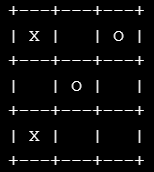
\includegraphics[width=0.6\textwidth]{sources/images/morpion_grille_exemple.png}\\
    \textit{Grille correspondant à \texttt{\{1,0,0,0,2,0,1,0,2\}}}
  \end{minipage}
\end{center}

Pour tester, déclarez le tableau et initialisez-le avec ces valeurs, puis affichez la grille pour vérifier (voir aide).

\subsection*{Cahier des charges}
\begin{UPSTICahierDesCharges}{1}
\begin{itemize}
  \item Boucle infinie munie d'un compteur de passages : si le compteur est pair, afficher \og joueur 1 joue \fg{}, sinon \og joueur 2 joue \fg{}. \textbf{Même code} pour les deux joueurs (c'est la variable \texttt{l\_joueur} qui fait la différence).
  \item Saisie de la case par le joueur \textbf{sans vérification} : affecter la case correspondante avec 1 (J1) ou 2 (J2).
  \item Afficher la grille après chaque coup.
\end{itemize}
\end{UPSTICahierDesCharges}

\begin{UPSTICahierDesCharges}{2}
\begin{itemize}
  \item Si la case n'existe pas ou est déjà occupée, le joueur \textbf{perd son tour} : la case n'est pas affectée et on passe au joueur suivant.
  \item \textbf{Détecter} la victoire : le joueur 1 gagne lorsque le \textbf{produit} des 3 cases d'une ligne, d'une colonne ou d'une diagonale vaut 1 ; le joueur 2 lorsqu'il vaut 8.
  \item \textbf{Détecter} la fin de partie sans vainqueur : le produit de toutes les cases est non nul.
\end{itemize}
\textit{Aide :} pensez à utiliser une ou plusieurs boucles \texttt{for} pour les tests.
\end{UPSTICahierDesCharges}

\begin{UPSTICahierDesCharges}{3}
\begin{itemize}
  \item Jouer contre l'ordinateur, muni d'une \textbf{intelligence artificielle} pour ne pas perdre et essayer de gagner.
  \item Écrire une fonction prenant en entrée le tableau de jeu et retournant 1 si le joueur 1 a gagné, 2 si le joueur 2 a gagné, -1 sinon. Demandez de l'aide à votre enseignant.
\end{itemize}
\end{UPSTICahierDesCharges}


\pagebreak
\section{Projet 8 — Puissance 4}
\setcounter{UPSTInumeroCahier des charges}{0}

\subsection*{Objectif du jeu}
Programmer un Puissance 4 sur une grille 6×6 en ASCII, jouable à deux, avec détection de 4 alignés.

\subsection*{Règles du jeu}
\begin{itemize}
  \item Une \textbf{grille 6×6} commune aux deux joueurs (1 et 2).
  \item À son tour, un joueur choisit une \textbf{colonne}; le pion tombe dans la \textbf{case libre la plus basse}.
  \item Afficher la grille après chaque coup. Le premier à aligner 4 pions gagne (—, | ou /).
\end{itemize}

\subsection*{Cahier des charges}
\begin{UPSTICahierDesCharges}{1}
\begin{itemize}
  \item Initialiser la grille à 0 et l’afficher.
  \item Boucle principale avec alternance J1/J2 et \textbf{choix d’une colonne} (sans validation initiale).
  \item Placer le pion en bas de la colonne, réafficher.
\end{itemize}
\end{UPSTICahierDesCharges}

\begin{UPSTICahierDesCharges}{2}
\begin{itemize}
  \item \textbf{Valider} la colonne (existence et place libre), sinon rejouer.
  \item Détecter \textbf{4 alignés} et l’égalité.
  \item Récapitulatif de fin.
\end{itemize}
\end{UPSTICahierDesCharges}

\begin{UPSTICahierDesCharges}{3}
\begin{itemize}
  \item Mode \textbf{joueur vs ordinateur} simple.
  \item Rejouabilité et présentation.
  \item Factoriser en fonctions (affichage, pose, test alignements).
\end{itemize}
\end{UPSTICahierDesCharges}


\pagebreak
\section{Projet 9 — Le bandit manchot}
\setcounter{UPSTInumeroCahier des charges}{0}

\subsection*{Objectif du jeu}
Simuler un bandit manchot (machines à sous) à 3 rouleaux et gérer le capital du joueur selon les combinaisons obtenues.


\subsection*{Règles du jeu}
\begin{itemize}
  \item 3 \textbf{rouleaux} de 11 figures (tableau 2D). Codes : \texttt{7, B, L, C} (sept, barre, citron, cerise).
  \item Le joueur commence avec \textbf{100 points} et mise 1 ou 3 points.
  \item Appui sur \texttt{J} : tirage aléatoire d’une figure par rouleau; affichage en ligne des trois codes.
  \item Le joueur gagne si une des combinaisons ci-dessous apparaît (\textbf{peu importe l'ordre}), sinon il perd sa mise ; le capital est mis à jour ; le joueur peut continuer (\texttt{O/N}).
\end{itemize}

\subsection*{Les rouleaux et les combinaisons}
\begin{center}
  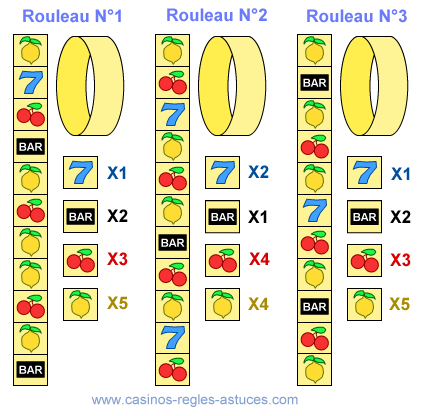
\includegraphics[width=0.7\textwidth]{sources/images/bandit_manchot_rouleaux.png}
\end{center}
Dans le programme : 7 est mémorisé par \texttt{'7'}, BAR par \texttt{'B'}, cerise par \texttt{'C'}, citron par \texttt{'L'}.

\textit{Conseils :} ranger les 3 figures tirées dans un tableau ; en mode test, vous pouvez modifier les rouleaux pour favoriser une combinaison.

\subsection*{Cahier des charges}
\begin{UPSTICahierDesCharges}{1}
\begin{itemize}
  \item Initialiser les \textbf{3 rouleaux} (tableau 3×11) et afficher leur contenu pour vérification.
  \item Tirer et afficher \textbf{une figure par rouleau} (codes).
  \item Mettre à jour le capital selon résultat simple (ex.\,égalité des 3).
\end{itemize}
\end{UPSTICahierDesCharges}

\begin{UPSTICahierDesCharges}{2}
\begin{itemize}
  \item Implémenter les \textbf{mises} (1 ou 3), détailler les combinaisons gagnantes/perdantes.
  \item Si aucune combinaison n'apparaît, le joueur peut \textbf{rejouer} un ou plusieurs rouleaux (ex.\,saisie \texttt{23} pour rejouer les rouleaux 2 et 3, puis \texttt{J}) ; il perd alors 1 point (ou 3 selon la mise de départ). Et ainsi de suite jusqu'à obtenir une combinaison ou ne plus avoir de points.
  \item Récapitulatif clair de fin.
\end{itemize}
\end{UPSTICahierDesCharges}

\begin{UPSTICahierDesCharges}{3}
\begin{itemize}
  \item Présentation et rejouabilité; options de test (rouleaux biaisés).
  \item Structuration en fonctions (tirage, calcul gain, affichage).
  \item Robustesse des saisies.
\end{itemize}
\end{UPSTICahierDesCharges}


\pagebreak
\section{Projet 10 — Le pendu}
\setcounter{UPSTInumeroCahier des charges}{0}

\subsection*{Objectif du jeu}
Faire deviner un mot lettre par lettre avec 7 erreurs autorisées, en affichant la progression.

\subsection*{Règles du jeu}
\begin{itemize}
  \item Un utilisateur saisit un \textbf{mot} (minuscule, sans accents ni espaces).
  \item Un joueur propose des lettres; le programme affiche le mot avec \_ pour les lettres non trouvées.
  \item À chaque lettre absente, \textbf{+1 erreur}. La partie s’arrête à 7 erreurs ou si le mot est trouvé.
  \item Variante 2 joueurs : inversion des rôles, 3 manches.
\end{itemize}

\subsection*{Cahier des charges}
\begin{UPSTICahierDesCharges}{1}
\begin{itemize}
  \item Saisir le mot \textbf{secret}, l’afficher \textbf{caractère par caractère} pour vérification, puis masquer.
  \item Boucle de jeu : saisie d’une lettre, mise à jour de l’affichage, \textbf{comptage des erreurs}.
  \item Condition de victoire/défaite.
\end{itemize}
\end{UPSTICahierDesCharges}

\begin{UPSTICahierDesCharges}{2}
\begin{itemize}
  \item Validation des saisies, gestion des lettres déjà proposées.
  \item Affichage du temps de jeu.
\end{itemize}
\end{UPSTICahierDesCharges}

\begin{UPSTICahierDesCharges}{3}
\begin{itemize}
  \item Présentation soignée -> Dessin ?
  \item Mode 2 joueurs avec alternance des rôles sur 3 manches.
  \item Option : dictionnaire de mots.
\end{itemize}
\end{UPSTICahierDesCharges}


\pagebreak
\section{Projet 11 — Mastermind -- Suite de couleurs}
\setcounter{UPSTInumeroCahier des charges}{0}

\subsection*{Objectif du jeu}
Deviner une suite cachée de 4 couleurs codées (0..3) avec indication des bien/mal placées.

\subsection*{Règles du jeu}
\begin{itemize}
  \item Le programme tire au hasard une \textbf{suite de 4 couleurs} parmi Rouge, Vert, Bleu, Noir (\textbf{avec répétitions possibles}).
  \item Codage : \texttt{0}=Noir, \texttt{1}=Rouge, \texttt{2}=Vert, \texttt{3}=Bleu.
  \item Le joueur saisit un \textbf{entier à 4 chiffres}; le programme le \textbf{décompose} en tableau.
  \item Le programme indique \textbf{nombre de bien placées} et \textbf{nombre de mal placées}. Score = tentatives × temps / 10.
\end{itemize}

\subsection*{Cahier des charges}
\begin{UPSTICahierDesCharges}{1}
\begin{itemize}
  \item Tirer la suite et \textbf{mémoriser} le code (tableau 4 cases); \textbf{ne pas l’afficher}.
  \item Le joueur saisit la proposition (entier 4 chiffres), \textbf{décomposer} en tableau, comparer et afficher les compteurs.
  \item Boucler jusqu’à la bonne réponse.
\end{itemize}
\end{UPSTICahierDesCharges}

\begin{UPSTICahierDesCharges}{2}
\begin{itemize}
  \item Gérer les répétitions correctement (bien/mal placées).
  \item Ajouter \textbf{chrono} et calcul du score; récapitulatif.
  \item Valider la saisie.
\end{itemize}
\end{UPSTICahierDesCharges}

\begin{UPSTICahierDesCharges}{3}
\begin{itemize}
  \item Mode \textbf{2 joueurs} en alternance; afficher les tentatives de chacun.
  \item Présentation (affichage de carrés ANSI) et rejouabilité.
  \item Factoriser en fonctions.
\end{itemize}
\end{UPSTICahierDesCharges}


\pagebreak
\section{Projet 12 — Black Jack adapté}
\setcounter{UPSTInumeroCahier des charges}{0}

\subsection*{Objectif du jeu}
Adapter un Black Jack simplifié avec un jeu de 52 cartes, tirage sans remise, calcul des scores et du gagnant. Le joueur 1 est un joueur physique, le joueur 2 est le programme.

\subsection*{Règles du jeu}
\begin{itemize}
  \item Jeu de \textbf{52 cartes} encodées \texttt{CCVV} (couleur$\times$100 + valeur). Couleurs : 72=\texttt{'H'} (c\oe{}ur), 80=\texttt{'P'} (pique), 84=\texttt{'T'} (trèfle), 67=\texttt{'C'} (carreau).
  \item Codes des cartes : 1 (As), 2, \ldots, 10, 11 (Valet), 12 (Dame), 13 (Roi).
  \item \textbf{Valeur} des cartes : 1 point pour l'As, 2 pour 2, \ldots, 9 pour 9, puis \textbf{10} pour 10, Valet, Dame et Roi.
  \item Le programme distribue \textbf{2 cartes} au joueur 1, additionne leurs valeurs et lui demande s'il en veut une autre. Il peut en demander autant qu'il veut, mais s'il dépasse 21, son score vaut 0 et il passe la main.
  \item Le joueur 2 (le programme) tire \textbf{autant de cartes} que le joueur 1. Le plus grand score gagne.
  \item Les cartes de chaque joueur sont rangées dans un tableau de 20 cases (pour être large).
\end{itemize}

\subsection*{Cahier des charges}
\begin{UPSTICahierDesCharges}{1}
\begin{itemize}
  \item Tirage des cartes \textbf{sans remise} : si au premier tirage (sur 52 cases) la case n°19 est choisie, on remplace son contenu par celui de la dernière case ; le tirage suivant se fait sur 51 cases \textit{(voir section~\ref{sec:tirage-sans-remise})}.
  \item Affichage des cartes tirées et proposition de tirer de nouvelles cartes.
  \item Calcul et affichage des scores, annonce du vainqueur.
\end{itemize}
\end{UPSTICahierDesCharges}

\begin{UPSTICahierDesCharges}{2}
\begin{itemize}
  \item En cas de match nul, une carte supplémentaire est tirée à chacun ; sa valeur s'ajoute à l'ancienne somme. Le vainqueur est celui qui obtient le plus grand score sans dépasser 21. Si les deux dépassent 21, c'est la somme de toutes les cartes qui départage.
\end{itemize}
\end{UPSTICahierDesCharges}

\begin{UPSTICahierDesCharges}{3}
\begin{itemize}
  \item Mode \textbf{2 joueurs}; comparaison et annonce du gagnant.
  \item Rejouabilité et présentation.
  \item Factoriser en fonctions.
\end{itemize}
\end{UPSTICahierDesCharges}


\pagebreak
\section{Projet 13 — Penalty !}
\setcounter{UPSTInumeroCahier des charges}{0}

\subsection*{Objectif du jeu}
Simuler une séance de tirs au but entre un joueur physique (joueur 1) et un joueur virtuel (joueur 2, le programme). Droite et gauche sont vues du côté du tireur.

\subsection*{Règles du jeu}
\begin{itemize}
  \item Le joueur 1 choisit un nom pour son équipe et un nom pour l'équipe du joueur 2.
  \item Le tireur choisit son tir sous la forme d'un caractère :
  \begin{itemize}
    \item \texttt{'d'} / \texttt{'g'} : à droite / à gauche du gardien, frappe molle et mal placée ;
    \item \texttt{'D'} / \texttt{'G'} : à droite / à gauche du gardien, frappe forte placée petit filet ;
    \item \texttt{'m'} : au milieu, frappe molle à ras de terre ; \texttt{'M'} : au milieu, frappe type panenka.
  \end{itemize}
  \item Les tirs \texttt{'D'}, \texttt{'G'} ou \texttt{'M'} ont $n$ chances sur 8 de terminer \textbf{en dehors de la cage}, où $n$ est le nombre de fois que \texttt{'D'}, \texttt{'G'} ou \texttt{'M'} ont déjà été choisis par ce joueur lors de la séance (tirage aléatoire par le programme).
  \item Le gardien plonge : \texttt{'d'} (à droite), \texttt{'g'} (à gauche) ou \texttt{'m'} (une partie du corps reste au milieu).
  \item Le gardien gagne si le tir est hors cadre, ou si le tir est \texttt{'d'}, \texttt{'g'} ou \texttt{'m'} et que le gardien a choisi respectivement \texttt{'d'}, \texttt{'g'} ou \texttt{'m'}. Sinon le tireur marque.
  \item Les choix du joueur virtuel sont aléatoires. Les joueurs changent de rôle après chaque tir.
  \item Séance de \textbf{5 penalties} tirés en alternance ; en cas d'égalité, \textbf{mort subite}. Le jeu s'arrête dès que l'issue est acquise (ex.\ 4 à 2 après 4 tirs).
\end{itemize}

\subsection*{Cahier des charges}
\begin{UPSTICahierDesCharges}{1}
\begin{itemize}
  \item Séance complète joueur physique contre programme : saisie des noms, choix des tirs et des plongeons, gestion de la probabilité de tir hors cadre, score.
  \item Fin anticipée de la séance, mort subite, annonce du vainqueur.
\end{itemize}
\end{UPSTICahierDesCharges}

\begin{UPSTICahierDesCharges}{2}
\begin{itemize}
  \item Ranger le résultat de chaque tir dans un tableau (un par joueur, 20 cases pour prévoir la mort subite) : 0 = manqué, 1 = arrêté par le gardien, 2 = réussi.
  \item En fin de partie, afficher le résumé de la séance \textbf{en couleur}, par exemple :
\begin{verbatim}
Penalty 1 pour OM : Arrêté par le gardien
Penalty 2 pour OM : Réussi
...
Penalty 5 pour PSG : Réussi

PSG win !!!
\end{verbatim}
\end{itemize}
\end{UPSTICahierDesCharges}

\begin{UPSTICahierDesCharges}{3}
\begin{itemize}
  \item Les 2 joueurs sont des joueurs physiques (choix du mode par menu).
\end{itemize}
\end{UPSTICahierDesCharges}

\pagebreak
\section{Projet 14 — Codenames}
\setcounter{UPSTInumeroCahier des charges}{0}

\subsection*{Objectif du jeu}
Mettre en place une version console de \textit{Codenames} permettant de jouer à deux équipes avec un plateau 5×5, un maître‑espion par équipe et une gestion claire des tours, révélations et conditions de fin.

\subsection*{Règles du jeu}
\begin{itemize}
  \item \textbf{Constitution du plateau} : 25 cartes (mots) sont placées en grille 5×5. Sous ces cartes se cachent des rôles : cartes \textbf{équipe Rouge}, cartes \textbf{équipe Bleue}, \textbf{neutres} et une carte \textbf{Assassin}. Une équipe commence (elle a une carte de plus).
  \item \textbf{Rôles} : chaque équipe a un \textbf{maître‑espion} (voit la carte‑clé indiquant la couleur de chaque mot) et des \textbf{agents} (devinent).
  \item \textbf{Tour de jeu} : le maître‑espion donne \textbf{un seul indice} (un mot) suivi d’un \textbf{nombre} indiquant combien de cartes de sa couleur sont visées. Les agents discutent et \textbf{désignent des cartes une par une}. Chaque désignation révèle la carte.
  \item \textbf{Révélations} : si la carte est de la couleur de l’équipe, elle reste au tour et peut continuer jusqu’à nombre + 1 maximum. Si elle est \textbf{neutre}, le tour s’arrête. Si elle est de la \textbf{couleur adverse}, le tour s’arrête et l’autre équipe marque la carte. Si c’est l’\textbf{Assassin}, l’équipe active \textbf{perd immédiatement}.
  \item \textbf{Fin de partie} : dès qu’une équipe a révélé toutes ses cartes, elle \textbf{gagne}. Si l’Assassin est révélé, l’autre équipe \textbf{gagne} aussitôt.
\end{itemize}

\subsection*{Cahier des charges}
\begin{UPSTICahierDesCharges}{1}
\begin{itemize}
  \item Le programme affiche la grille
  \item Le programme demande puis affiche une carte espions pour les que les espions la connaissent
  \item Une touche permet de cacher la carte espion
\end{itemize}
\end{UPSTICahierDesCharges}

\begin{UPSTICahierDesCharges}{2}
\begin{itemize}
  \item On peut choisir une case, la case est alors cachée et remplacée par le numéro de l'équipe à laquelle elle correspond
\end{itemize}
\end{UPSTICahierDesCharges}

\begin{UPSTICahierDesCharges}{3}
\begin{itemize}
  \item Gestion automatique des tours de jeu
\end{itemize}
\end{UPSTICahierDesCharges}

\pagebreak
\section{Projet 15 — 2048}
\setcounter{UPSTInumeroCahier des charges}{0}

\subsection*{Objectif du jeu}
Faire glisser et fusionner les tuiles d'une grille $4\times4$ pour obtenir une tuile de valeur \textbf{2048}.

\subsection*{Règles du jeu}
\begin{itemize}
  \item La grille est un \textbf{tableau 2D d'entiers} $4\times4$ ; une case vide contient \texttt{0}.
  \item Au départ, \textbf{2 tuiles de valeur 2} sont placées au hasard sur deux cases vides \textbf{distinctes}.
  \item À chaque coup, le joueur choisit une direction : \texttt{8}/\texttt{2}/\texttt{4}/\texttt{6} (pavé numérique) ou \texttt{z}/\texttt{s}/\texttt{q}/\texttt{d} pour haut/bas/gauche/droite.
  \item Toutes les tuiles \textbf{glissent} dans cette direction jusqu'au bord ou jusqu'à une autre tuile.
  \item Deux tuiles adjacentes \textbf{de même valeur} dans le sens du mouvement \textbf{fusionnent} en une tuile de valeur double. Une tuile ne fusionne \textbf{qu'une seule fois par coup} (pas de fusion en chaîne : la ligne \texttt{2 2 4 0} poussée à gauche donne \texttt{4 4 0 0}, et non \texttt{8 0 0 0}).
  \item Si le coup a \textbf{modifié la grille}, une nouvelle tuile (\texttt{2} ou \texttt{4}, au hasard) apparaît sur une case vide.
  \item \textbf{Victoire} dès qu'une tuile atteint 2048. \textbf{Défaite} si la grille est pleine et qu'aucune direction ne peut plus la modifier.
\end{itemize}

\textit{Conseil :} commencer par traiter une \textbf{seule ligne} vers la gauche (tableau 1D de 4 cases) : on tasse d'abord les valeurs non nulles vers la gauche (décalage), on fusionne les paires voisines égales, puis on tasse à nouveau. Les trois autres directions se ramènent à ce cas en parcourant la grille dans un autre ordre.

\subsection*{Cahier des charges}
\begin{UPSTICahierDesCharges}{1}
\begin{itemize}
  \item Déclarer la grille $4\times4$ et l'\textbf{initialiser à 0}.
  \item Placer \textbf{2 tuiles de valeur 2} sur deux cases vides distinctes tirées au hasard.
  \item \textbf{Afficher} la grille proprement (colonnes alignées, \texttt{.} pour une case vide).
\end{itemize}
\end{UPSTICahierDesCharges}

\begin{UPSTICahierDesCharges}{2}
\begin{itemize}
  \item Écrire le \textbf{glissement + fusion vers la gauche}, ligne par ligne, en respectant la règle « une seule fusion par tuile et par coup ».
  \item Tester sur des lignes choisies à la main (\texttt{2 2 2 2} $\rightarrow$ \texttt{4 4 0 0}, \texttt{0 2 0 2} $\rightarrow$ \texttt{4 0 0 0}, \texttt{4 2 2 0} $\rightarrow$ \texttt{4 4 0 0}).
  \item Indiquer si le coup a \textbf{modifié} la grille (comparaison avant/après).
\end{itemize}
\end{UPSTICahierDesCharges}

\begin{UPSTICahierDesCharges}{3}
\begin{itemize}
  \item Gérer les \textbf{4 directions} et la saisie du joueur (refuser une touche invalide).
  \item Ajouter une \textbf{nouvelle tuile} (2 ou 4) après chaque coup valide uniquement.
  \item Détecter la \textbf{victoire} (tuile 2048) et la \textbf{défaite} (grille pleine et aucun coup possible) ; structurer en fonctions.
\end{itemize}
\end{UPSTICahierDesCharges}

\textit{Amélioration :} score cumulé (somme des valeurs créées par fusion) ; affichage \textbf{couleur} selon la valeur de la tuile avec les codes ANSI \texttt{\textbackslash033[4Xm} déjà vus dans les projets 5 et 11.


\pagebreak
\section{Projet 16 — Le taquin}
\setcounter{UPSTInumeroCahier des charges}{0}

\subsection*{Objectif du jeu}
Remettre dans l'ordre les nombres 1 à 15 d'une grille $4\times4$ en faisant glisser les tuiles dans la case vide.

\subsection*{Règles du jeu}
\begin{itemize}
  \item La grille est un \textbf{tableau 2D d'entiers} $4\times4$ contenant les nombres \texttt{1} à \texttt{15} et une \textbf{case vide codée \texttt{0}}.
  \item Le joueur désigne une tuile \textbf{adjacente} à la case vide (par sa valeur, ou par une direction) ; adjacente signifie au-dessus, en dessous, à gauche ou à droite (pas en diagonale).
  \item Si la tuile est bien adjacente, elle \textbf{échange sa position} avec la case vide ; sinon le coup est refusé.
  \item Le jeu est \textbf{gagné} lorsque les tuiles sont rangées dans l'ordre croissant, ligne par ligne, la case vide étant en bas à droite.
\end{itemize}

\textit{Attention :} remplir la grille par un mélange totalement aléatoire des 16 valeurs produit, une fois sur deux, un taquin \textbf{impossible à résoudre}. On part donc de la grille triée et on effectue une longue série de \textbf{déplacements valides} tirés au hasard : la grille obtenue est toujours soluble. Le déplacement lui-même n'est qu'un \textbf{échange} de deux cases, comme dans le tirage sans remise (section~\ref{sec:tirage-sans-remise}).

\subsection*{Cahier des charges}
\begin{UPSTICahierDesCharges}{1}
\begin{itemize}
  \item Initialiser la grille \textbf{triée} (\texttt{1..15} puis \texttt{0}) et l'\textbf{afficher} (case vide affichée par un espace).
  \item Écrire une fonction qui retrouve la \textbf{position (ligne, colonne)} de la case vide.
\end{itemize}
\end{UPSTICahierDesCharges}

\begin{UPSTICahierDesCharges}{2}
\begin{itemize}
  \item \textbf{Mélanger} la grille par une série (par ex.\,200) d'échanges valides aléatoires de la case vide avec une voisine.
  \item Demander au joueur la tuile à déplacer, vérifier qu'elle est \textbf{adjacente} à la case vide, puis effectuer l'\textbf{échange} ; sinon afficher un message d'erreur.
  \item Ré-afficher la grille après chaque coup.
\end{itemize}
\end{UPSTICahierDesCharges}

\begin{UPSTICahierDesCharges}{3}
\begin{itemize}
  \item Détecter la \textbf{victoire} par comparaison avec la grille triée.
  \item Compter et afficher le \textbf{nombre de coups} joués.
  \item Structurer en fonctions (affichage, recherche de la case vide, déplacement, test de victoire) et sécuriser les saisies.
\end{itemize}
\end{UPSTICahierDesCharges}

\textit{Amélioration :} chronométrer la partie avec \texttt{time(NULL)} (voir section Bonus) et afficher le temps de résolution.


\pagebreak
\section{Projet 17 — Memory}
\setcounter{UPSTInumeroCahier des charges}{0}

\subsection*{Objectif du jeu}
Retrouver les 8 paires de valeurs identiques cachées dans une grille de 16 cases, en un minimum de tentatives.

\subsection*{Règles du jeu}
\begin{itemize}
  \item La grille compte \textbf{16 cases} ($4\times4$, tableau d'entiers ou de \texttt{char}) contenant \textbf{8 paires} : les valeurs \texttt{1} à \texttt{8}, chacune en double, placées au hasard.
  \item Par défaut toutes les cases sont \textbf{cachées} et affichées \texttt{?}.
  \item À chaque tentative, le joueur indique \textbf{deux positions distinctes} ; leurs valeurs sont révélées.
  \item Si les deux valeurs sont \textbf{identiques}, la paire est trouvée et reste visible définitivement ; sinon les deux cases sont de nouveau cachées après une courte pause (\texttt{sleep()}, voir section Bonus).
  \item Le jeu est \textbf{gagné} lorsque les 8 paires sont trouvées.
\end{itemize}

\textit{Conseil :} on utilise deux tableaux de même taille : l'un contient les \textbf{valeurs}, l'autre l'\textbf{état} de chaque case (trouvée ou non). Le mélange initial repose sur des échanges de cases, comme le tirage sans remise (section~\ref{sec:tirage-sans-remise}).

\subsection*{Cahier des charges}
\begin{UPSTICahierDesCharges}{1}
\begin{itemize}
  \item Remplir la grille avec les valeurs \texttt{1} à \texttt{8} \textbf{en double}.
  \item \textbf{Mélanger} la grille aléatoirement par échanges de cases.
  \item Afficher la grille \textbf{cachée} (\texttt{?}) ; en mode test, afficher aussi la grille réelle.
\end{itemize}
\end{UPSTICahierDesCharges}

\begin{UPSTICahierDesCharges}{2}
\begin{itemize}
  \item Saisir \textbf{deux positions} (vérifier qu'elles sont valides, distinctes et non déjà trouvées).
  \item Afficher \textbf{temporairement} les deux valeurs réelles, puis les \textbf{comparer}.
  \item Mettre à jour le \textbf{tableau d'état} (case trouvée oui/non) et ré-afficher la grille après la pause.
\end{itemize}
\end{UPSTICahierDesCharges}

\begin{UPSTICahierDesCharges}{3}
\begin{itemize}
  \item Compter et afficher le \textbf{nombre de tentatives}.
  \item Détecter la \textbf{victoire} (8 paires sur 8).
  \item Structurer en fonctions (remplissage, mélange, affichage, saisie, comparaison).
\end{itemize}
\end{UPSTICahierDesCharges}

\textit{Amélioration :} mode \textbf{2 joueurs} : le joueur qui trouve une paire rejoue ; le vainqueur est celui qui a trouvé le plus de paires.


\pagebreak
\section{Tirage \emph{sans remise}}
\label{sec:tirage-sans-remise}

% Marqueur pédagogique caché (texte blanc sur fond blanc). Source unique
% du texte : sources/images/marqueur_qr.txt (le QR en pied de page, voir
% td_tableaux.tex, encode ce même fichier -- modifier uniquement ce .txt
% puis régénérer le QR, voir le commentaire dans td_tableaux.tex).
\noindent\textcolor{white}{\input{sources/images/marqueur_qr.txt}}


\subsection*{Idée générale}
On veut tirer des éléments \textbf{sans jamais retomber deux fois sur le même} (par exemple, des cartes d’un paquet).  
Le principe le plus simple et robuste consiste à :
\begin{enumerate}
  \item Stocker tous les éléments dans un tableau (paquet).
  \item À chaque tirage $k$, \textbf{tirer un index aléatoire} parmi les positions encore disponibles $[0\,..\,\texttt{borne}]$.
  \item \textbf{Échanger} l’élément tiré avec celui en fin de zone disponible (\texttt{borne}), puis \textbf{réduire la borne} d’1.
\end{enumerate}
Ainsi, la zone \texttt{[0..borne]} contient encore les cartes disponibles, et la zone \texttt{[borne+1..fin]} contient les cartes déjà tirées.

\subsection*{Schéma visuel pas à pas}
Exemple avec 6 cartes initiales : \texttt{[A, B, C, D, E, F]} (indices \texttt{0..5}), \texttt{borne = 5}.

\paragraph{Tirage \#1} on tire un index aléatoire \texttt{i = 2} (la carte \texttt{C}) dans \texttt{[0..5]}.
\[
\begin{array}{c|c|c|c|c|c}
\texttt{0} & \texttt{1} & \color{blue}{\texttt{2}} & \texttt{3} & \texttt{4} & \texttt{5}\\
\boxed{\texttt{A}} & \boxed{\texttt{B}} & \boxed{\texttt{C}} & \boxed{\texttt{D}} & \boxed{\texttt{E}} & \boxed{\texttt{F}} \\
\hline
\end{array}
\]
On \textbf{échange} la case \texttt{i=2} avec la case \texttt{borne=5} :
\[
\begin{array}{c|c|c|c|c|c}
\texttt{0} & \texttt{1} & \color{blue}{\texttt{2}} & \texttt{3} & \texttt{4} & \color{gray}{\texttt{5}}\\
\boxed{\texttt{A}} & \boxed{\texttt{B}} & \boxed{\texttt{F}} & \boxed{\texttt{D}} & \boxed{\texttt{E}} & \fbox{\texttt{C}} \\
\hline
\end{array}
\]
Puis \texttt{borne ← 4}. La carte \texttt{C} est « sortie » (à droite), elle ne sera plus retirable.

\paragraph{Tirage \#2} on tire \texttt{i = 1} dans \texttt{[0..4]} (car \texttt{borne=4}) :
\[
\begin{array}{c|c|c|c|c|c}
\texttt{0} & \color{blue}{\texttt{1}} & \texttt{2} & \texttt{3} & \color{gray}{\texttt{4}} & \color{gray}{\texttt{5}}\\
\boxed{\texttt{A}} & \boxed{\color{blue}{\texttt{B}}} & \boxed{\texttt{F}} & \boxed{\texttt{D}} & \boxed{\texttt{E}} & \fbox{\texttt{C}} \\
\hline
\end{array}
\]
On \textbf{échange} avec \texttt{borne=4}, puis \texttt{borne ← 3} :
\[
\begin{array}{c|c|c|c|c|c}
\texttt{0} & \texttt{1} & \texttt{2} & \texttt{3} & \color{gray}{\texttt{4 (tirée)}} & \color{gray}{\texttt{5 (tirée)}}\\
\boxed{\texttt{A}} & \boxed{\texttt{E}} & \boxed{\texttt{F}} & \boxed{\texttt{D}} & \fbox{\texttt{B}} & \fbox{\texttt{C}} \\
\hline
\end{array}
\]
On poursuit ainsi jusqu’à ce que \texttt{borne < 0} (toutes les cartes tirées), ou qu’on ait tiré le nombre voulu de cartes.

% \subsection*{Invariants et garanties}
% \begin{itemize}
%   \item \textbf{Uniformité} : à chaque tirage, tous les éléments encore disponibles ont la même probabilité d’être choisis (car on choisit l’index \texttt{i} uniformément dans \texttt{[0..borne]}).
%   \item \textbf{Sans doublon} : un élément tiré est \textbf{sorti} de la zone \texttt{[0..borne]} ; il ne peut plus être re-tiré.
%   \item \textbf{Coût linéaire} : chaque tirage fait au plus un échange (opération \texttt{O(1)}) ; tirer $K$ cartes coûte \texttt{O(K)}.
% \end{itemize}

% \subsection*{Façons d’utiliser l’idée}
% \paragraph{(A) Tirer quelques cartes seulement.}
% On répète le processus $K$ fois (avec $K \le$ taille du paquet). À chaque fois, on choisit \texttt{i} dans \texttt{[0..borne]}, on échange, puis \texttt{borne ← borne - 1}.

% \paragraph{(B) Mélanger (shuffle) entièrement.}
% On applique la même logique en parcourant \texttt{borne} de la fin vers le début :
% \begin{enumerate}
%   \item Pour \texttt{borne = n-1} jusqu’à \texttt{1} :
%   \item \quad tirer \texttt{i} uniformément dans \texttt{[0..borne]} et échanger les cases \texttt{i} et \texttt{borne}.
% \end{enumerate}
% Au final, le tableau est un \textbf{mélange uniforme} (algorithme de Fisher–Yates).

% \subsection*{Exemple de squelette (C) pour \emph{tirer $K$ éléments sans remise}}
% \begin{lstlisting}[language=C]
% // l_tab contient N éléments disponibles
% // borne marque la limite de la zone encore "tirable"
% int borne = N - 1;

% for (int tir = 0; tir < K; tir++) {
%     // index aléatoire uniforme dans [0..borne]
%     int i = rand() % (borne + 1);

%     // récupérer l'élément tiré
%     int carte = l_tab[i];

%     // échanger l_tab[i] avec l_tab[borne] pour "sortir" la carte
%     int tmp = l_tab[i];
%     l_tab[i] = l_tab[borne];
%     l_tab[borne] = tmp;

%     // la carte tirée est désormais en fin de zone
%     // (on peut la stocker, l'afficher, etc.)
%     printf("Tirage #%d : %d\n", tir+1, carte);

%     // réduire la zone disponible
%     borne--;
% }
% \end{lstlisting}

\subsection*{Erreurs fréquentes à éviter}
\begin{itemize}
  \item \textbf{Ne pas réduire la borne} $\Rightarrow$ risque de re-tirer la même carte.
  \item \textbf{Tirer sur toute la longueur} \texttt{[0..N-1]} à chaque fois $\Rightarrow$ doublons possibles.
  \end{itemize}


\end{document}